\scanpage{129}
% archive sheet number: 128
% top marginal question
\margin{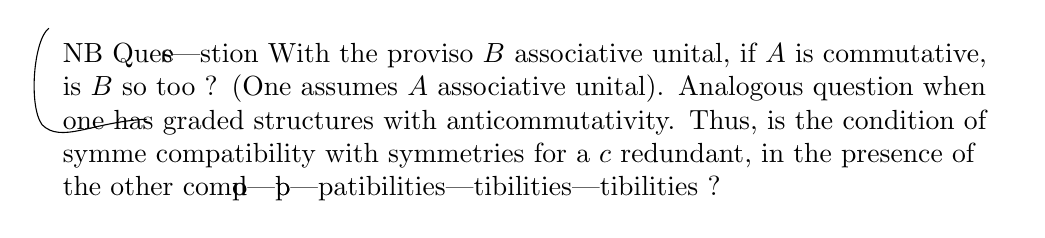
\begin{tikzpicture}[x=.35cm,y=.35cm,baseline=(n.base)]\node[anchor=north west,align=left,text width=12cm] (n) at (.6,0) {\handwritten{\uline{NB}} \uline{Que\unsure{\rlap{e}s|s}tion} With the proviso $B$ associative unital, if $A$ is commutative, is $B$ so too ? (One assumes $A$ associative unital). Analogous question when one has graded structures with anticommutativity. Thus, is the condition of \deleted{symme} compatibility with symmetries for a $c$ redundant, in the presence of the other com\unsure{\rlap{d}p|\rlap{b}p|p}a\unsure{t\handwritten{ibilities}|t\handwritten{ibilities}|tibilities} ?};\draw (.45,.2) .. controls (-.1,-.2) and (-.3,-2.6) .. (.2,-3.3) .. controls (.9,-4) and (2,-3.2) .. (4,-3.1);\end{tikzpicture}}
% source lines 1--3
of faithfully flat base $k'\handwritten{\longrightarrow}B$, \deleted{the functor} it becomes trivial, so one has a ``torsor'' under the monoid $\unsure{\rlap{\(G\)}H|\mathbb H|\mathbb G}_{k'}$ ; then the new fiber functor $G$ is deduced from $F'=F\unsure{\otimes|\Omega}_k k'$ by twisting using $G$ \ldots

% source lines 4--14
But suppose on\deleted{e}ly $A$ an associative unital algebra, and $B$ ditto, with no commutativity condition.\inserted{One assumes $A$ with \uline{antipode}\inserted{\handwritten{$\underline{a}$}} (do without it ?).}\handwritten{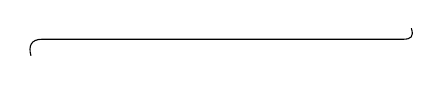
\begin{tikzpicture}[x=.35cm,y=.35cm,baseline=-.2ex]\draw (0,-.5) .. controls (-.1,-.15) and (0,.1) .. (.4,.1)--(13.5,.1) .. controls (13.8,.1) and (13.9,.2) .. (13.8,.5);\end{tikzpicture}} Let us take a $\handwritten{\sigma\in}U\otimes_k U$ \deleted{abov} as above to introduce a commutativity relation $\handwritten{\unsure{\psi|\phi}}$ . Let us note (except that $k'$ is no longer assumed to be a field) one finds a category $C'=C\otimes_k k'$ over $k'$, with $\otimes$, defined\inserted{\handwritten{(either by $U'$, \uuline{or} dually)}}\handwritten{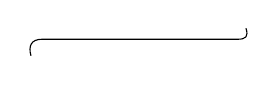
\begin{tikzpicture}[x=.35cm,y=.35cm,baseline=-.2ex]\draw (0,-.5) .. controls (-.1,-.15) and (0,.1) .. (.4,.1)--(7.5,.1) .. controls (7.8,.1) and (7.9,.2) .. (7.8,.5);\end{tikzpicture}} by the ``pro-ring'' $V=G(U)=L\overset{\handwritten{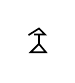
\begin{tikzpicture}[x=.35cm,y=.35cm,baseline=-.2ex]\draw[line width=.6pt] (0,0)--(.3,.3)--(.55,0)--cycle;\draw (.3,.3)--(.3,.65);\draw[line width=.6pt] (-.08,.62)--(.3,.86)--(.52,.64)--(.12,.64);\end{tikzpicture}}}{\otimes}_U(U,\mathrm{int})$, where $(U,\mathrm{int})$ denotes $U$ equipped with the structure of a $U$-module \deleted{(hence of a pro-object of} (and even of a ``pro-ring'' object (for $\otimes$) of $C$) defined using its bimodule structure over $U^o\overset{\handwritten{\scriptscriptstyle\wedge}}{\otimes} U$ \deleted{using} by restriction of scalars via $U\handwritten{\xrightarrow{\Delta}}U\overset{\handwritten{\scriptscriptstyle\wedge}}{\otimes} U\handwritten{\xrightarrow{\underline a\otimes\mathrm{id}_U}}U^o\overset{\handwritten{\scriptscriptstyle\wedge}}{\otimes} U$ : Twisting by $L$ and using the fact that one has compatibility with $\otimes$, one finds a pro-ring $V$ over $k'$, and the latter inherits from $U$ a diagonal map \ldots
\margin{\handwritten{?}}
% left margin, a), alongside source lines 9--16
\margin{\handwritten{a) give an intrinsic meaning : $C\otimes_k k'$, independently of \deleted{$\unsure{\circ|\otimes}$} the datum of $F$ (\uline{NB} if $k'$ is not a field, it is not an \uline{abelian} category, only additive)}}
% source lines 15--29
That\deleted{\unsure{s|x}} said, if one has a datum $\handwritten{\sigma\in}U\overset{\handwritten{\scriptscriptstyle\wedge}}{\otimes} U$ satisfying conditions (1)\inserted{above,}\handwritten{\begin{tikzpicture}[x=.35cm,y=.35cm,baseline=-.2ex]\draw (0,-.5) .. controls (-.1,-.15) and (0,.1) .. (.4,.1)--(4.5,.1) .. controls (4.8,.1) and (4.9,.2) .. (4.8,.5);\end{tikzpicture}} can one define in terms of $\handwritten{\sigma}$ (or does there at least exist) an element $\handwritten{\tau\in}V\overset{\handwritten{\scriptscriptstyle\wedge}}{\otimes}_k V$ satisfying the relations analogous to (1), in such a way that $(G,c)$ is compatible with the symmetr\unsure{\rlap{t}y|y} isomorphisms $\handwritten{\psi}$ in $C$ d\unsure{e|e}fined by $\handwritten{\sigma}$, $\handwritten{\psi'}$ in $C'$ defined by $\handwritten{\tau}$ ??? The only chance of \deleted{showing it} constructing a $\handwritten{\tau}$ canonically seems to be to prove that $\handwritten{\tau}$ is ``invariant'' when one lets $U$ act on $U\overset{\handwritten{\scriptscriptstyle\wedge}}{\otimes}_k U=(U,\mathrm{int})\overset{\handwritten{\scriptscriptstyle\wedge}}{\otimes}(U,\mathrm{int})$ by means of its \deleted{e}action mentioned above on the two factors, which is expressed by the relation $U^+ .\handwritten{\unsure{\tau^{\scriptscriptstyle\cdot}|\tau'|\tau}}=0$.\inserted{\handwritten{[Check in the graded case what happens !]}}\handwritten{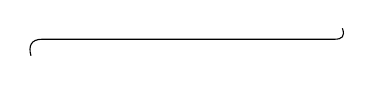
\begin{tikzpicture}[x=.35cm,y=.35cm,baseline=-.2ex]\draw (0,-.5) .. controls (-.1,-.15) and (0,.1) .. (.4,.1)--(11.0,.1) .. controls (11.3,.1) and (11.4,.2) .. (11.3,.5);\end{tikzpicture}} - If this worked (which would improve the result wan\deleted{t}ted in NB at the top of the page), this would show that in the study of fibre functors, there is reason to drop the questions of compatibility with symmetries, these always being recovered afterwards.\inserted{\handwritten{(But, cf examples numbe\textsuperscript{r} 1\unsure{2|1}).}}
% left margin, b), alongside source lines 17--21
\margin{\handwritten{b) Show that structure $\unsure{\ominus|\otimes}$, possibly with data $\varphi,\psi,1,\vee$. extends automatically to $C'$, with its axioms}}
% left margin, c), alongside source lines 22--30
\margin{\handwritten{c) generalize, for a functor such as $G:C\to\mathrm{Mod}(k')$, the description of numbe\textsuperscript{r} 6 into a description of $C'$ in terms of a pro-ring $U'=\mathrm{End}(G)$, and make explicit how one still has the various structures on $C$: $\otimes,\varphi,\psi,1,\vee$}}

% source lines 30--31; word continues on scan 130
There would then remain the question of an \uline{intrinsic} description of a category $C$ as in numbe\textsuperscript{r} 1,\inserted{\handwritten{with $\check{X}$}}\handwritten{\begin{tikzpicture}[x=.35cm,y=.35cm,baseline=-.2ex]\draw (0,-.5) .. controls (-.1,-.15) and (0,.1) .. (.4,.1)--(2.6,.1) .. controls (2.9,.1) and (3.0,.2) .. (2.9,.5);\end{tikzpicture}} indepen\unsure{\rlap{e}d|d}\unsure{\rlap{m}e|\rlap{n}e|e}\unsure{\rlap{e}n|n}\unsure{\rlap{n}t|t}ly of the datum of an $F$ preli%
